\documentclass[tikz,border=8pt]{standalone}
\usepackage{xcolor}
\usetikzlibrary{arrows.meta,positioning}
\tikzset{
  head/.style={
    draw,
    rounded corners=4pt,
    minimum width=4.9cm,
    minimum height=0.95cm,
    text width=4.7cm,
    align=center,
    font=\small\bfseries,
    fill=gray!10
  },
  ws/.style={
    draw,
    rounded corners=4pt,
    minimum width=4.2cm,
    minimum height=0.9cm,
    text width=4.0cm,
    align=center,
    font=\scriptsize,
    fill=blue!8
  },
  http/.style={
    draw,
    rounded corners=4pt,
    minimum width=4.2cm,
    minimum height=0.9cm,
    text width=4.0cm,
    align=center,
    font=\scriptsize,
    fill=green!9
  },
  store/.style={
    draw,
    rounded corners=4pt,
    minimum width=4.2cm,
    minimum height=0.9cm,
    text width=4.0cm,
    align=center,
    font=\scriptsize,
    fill=orange!12
  },
  flow/.style={->, >=Latex, thick, draw=gray!70}
}
\begin{document}
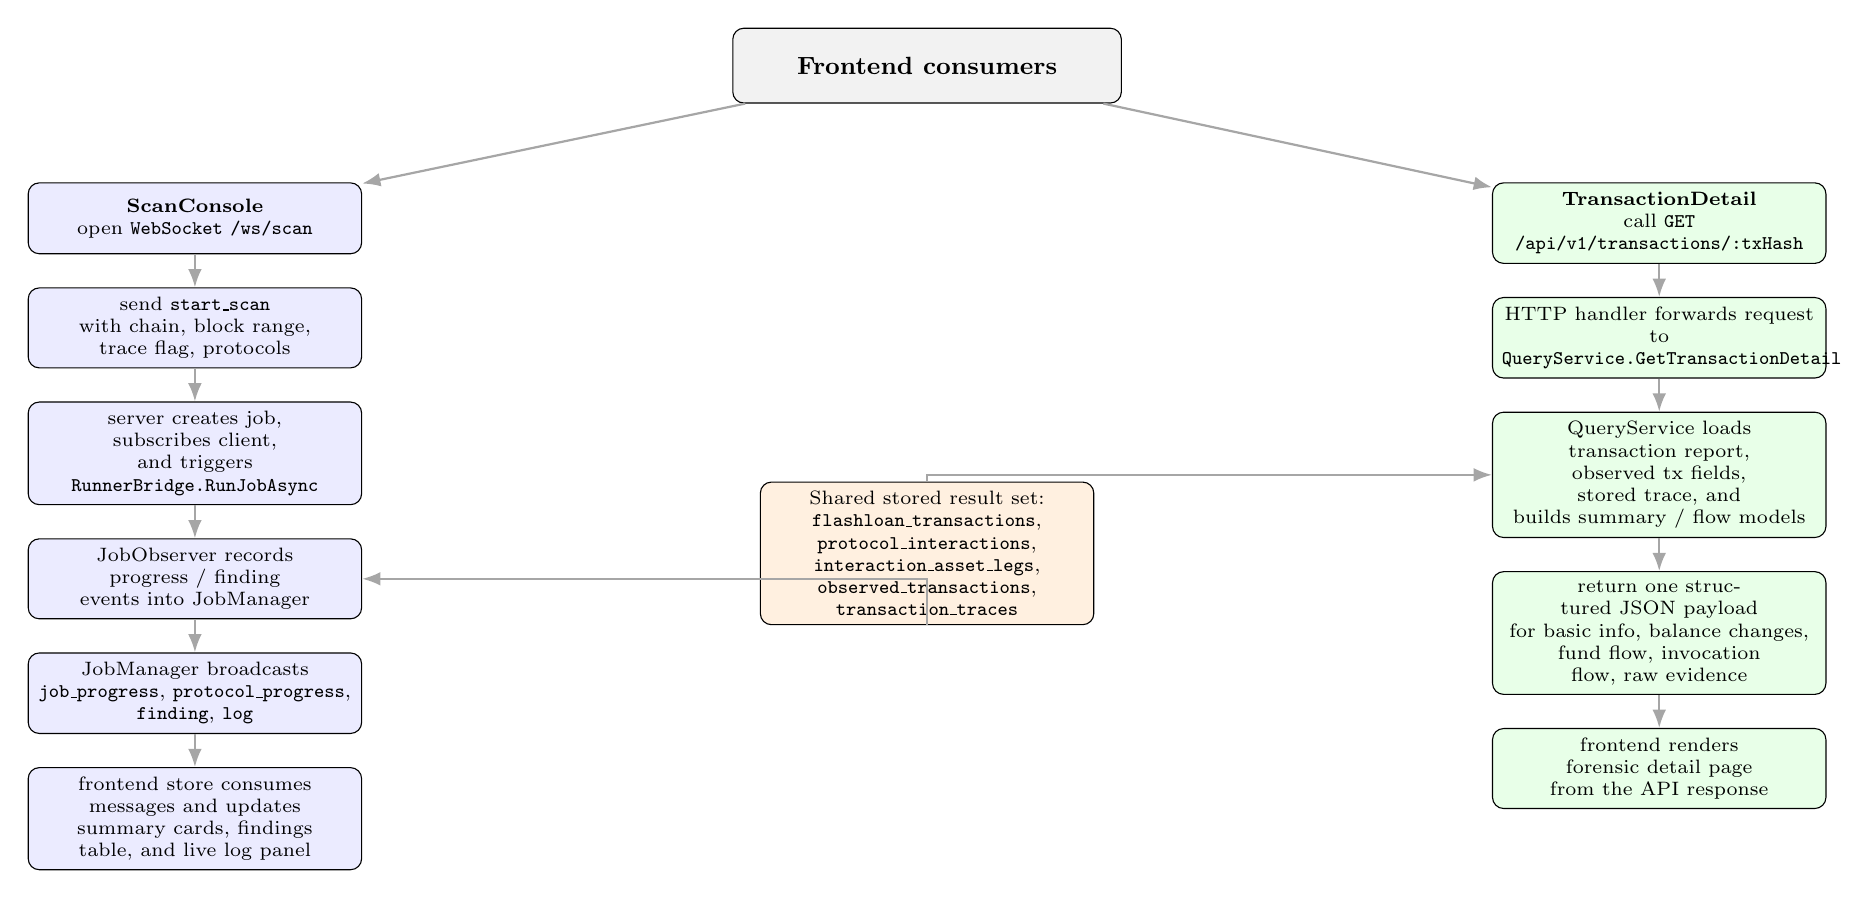
\begin{tikzpicture}[node distance=0.42cm]
  \node[head] (front) at (0,0) {Frontend consumers};

  \node[ws, below left=1.0cm and 4.7cm of front] (ws1) {\textbf{ScanConsole}\\open \texttt{WebSocket /ws/scan}};
  \node[ws, below=of ws1] (ws2) {send \texttt{start\_scan}\\with chain, block range, trace flag, protocols};
  \node[ws, below=of ws2] (ws3) {server creates job, subscribes client,\\and triggers \texttt{RunnerBridge.RunJobAsync}};
  \node[ws, below=of ws3] (ws4) {JobObserver records progress / finding\\events into JobManager};
  \node[ws, below=of ws4] (ws5) {JobManager broadcasts\\\texttt{job\_progress}, \texttt{protocol\_progress},\\\texttt{finding}, \texttt{log}};
  \node[ws, below=of ws5] (ws6) {frontend store consumes messages and updates\\summary cards, findings table, and live log panel};

  \node[http, below right=1.0cm and 4.7cm of front] (h1) {\textbf{TransactionDetail}\\call \texttt{GET /api/v1/transactions/:txHash}};
  \node[http, below=of h1] (h2) {HTTP handler forwards request\\to \texttt{QueryService.GetTransactionDetail}};
  \node[http, below=of h2] (h3) {QueryService loads transaction report,\\observed tx fields, stored trace, and\\builds summary / flow models};
  \node[http, below=of h3] (h4) {return one structured JSON payload\\for basic info, balance changes,\\fund flow, invocation flow, raw evidence};
  \node[http, below=of h4] (h5) {frontend renders forensic detail page\\from the API response};

  \node[store, below=4.8cm of front] (db) {Shared stored result set:\\\texttt{flashloan\_transactions}, \texttt{protocol\_interactions},\\\texttt{interaction\_asset\_legs}, \texttt{observed\_transactions}, \texttt{transaction\_traces}};

  \draw[flow] (front) -- (ws1);
  \draw[flow] (front) -- (h1);

  \draw[flow] (ws1) -- (ws2);
  \draw[flow] (ws2) -- (ws3);
  \draw[flow] (ws3) -- (ws4);
  \draw[flow] (ws4) -- (ws5);
  \draw[flow] (ws5) -- (ws6);

  \draw[flow] (h1) -- (h2);
  \draw[flow] (h2) -- (h3);
  \draw[flow] (h3) -- (h4);
  \draw[flow] (h4) -- (h5);

  \draw[flow] (db) |- (ws4);
  \draw[flow] (db) |- (h3);
\end{tikzpicture}
\end{document}
